\documentclass[12pt, a4paper]{article}
\usepackage[spanish]{babel}
\usepackage{geometry}
\usepackage[utf8]{inputenc}
\usepackage{lipsum} % Para texto de ejemplo (puedes eliminarlo)
% Remover numeración en secciones
\setcounter{secnumdepth}{-1} % Place this in the preamble

% Set sans-serif font
\usepackage{lmodern}
\renewcommand{\familydefault}{\sfdefault}

% Remover numeración en indice
\usepackage{titlesec}
\usepackage{tocloft}
\renewcommand{\cftsecnumwidth}{0pt}   % Hide section numbers in TOC
\renewcommand{\cftsecaftersnum}{}     % Remove space after section numbers

% Configuración básica de la página
\geometry{a4paper, margin=2.5cm}

% Comando para citar
\newcommand{\miCita}[1]{\cite{#1}}

% Configuración de las referencias
\usepackage[natbibapa]{apacite}
\renewcommand{\bibliographytypesize}{\small}
\AtBeginDocument{\renewcommand{\refname}{Referencias}}

\usepackage{graphicx}
\graphicspath{{/home/ddominguez/Documents/School/7/Sem_BD/Proyecto_Final/}}

% Paquetes para escribir código SQL
\usepackage{listings}
\usepackage{xcolor}
\lstset{
  language=SQL,
  basicstyle=\ttfamily\small,
  keywordstyle=\color{blue}\bfseries,
  stringstyle=\color{red!70!black},
  commentstyle=\color{gray}\itshape,
  columns=flexible,
  breaklines=true,
  showstringspaces=false,
  backgroundcolor=\color{gray!10},
  frame=single
}

% Insertar documentos PDF
\usepackage{pdfpages}

\begin{document}
\begin{titlepage}
\end{titlepage}

% ------------------------------------------------------------------------------
\begin{titlepage}
\begin{center}
 {\Huge\bfseries Reporte del Proyecto Final\\}
 \vspace{1cm}

 {\huge 17/05/25\\}
 \vspace{2cm}

 {\Large\bfseries Diego Martín Domínguez Hernández}\\[5pt]
 \vspace{2cm}

 {\Large Seminario de bases de datos}\\[5pt]
 \vspace{2cm}

 {\Large Prof. José Antonio Aviña Mendez}\\[5pt]
\end{center}
\end{titlepage}

\newpage
\tableofcontents
\newpage

\section{Introducción}
Las bibliotecas son el pilar fundamental del conocimiento y el aprendizaje; sin embargo, en la era digital, se enfrentan nuevos retos y oportunidades. Este proyecto busca responder a estos desafíos mediante un sistema integral de gestión de bases de datos diseñado específicamente para bibliotecas modernas. El sistema tiene como objetivo optimizar las operaciones bibliotecarias, incluyendo la gestión del inventario de libros, el registro de usuarios, el seguimiento de préstamos y la administración de reservas. Esta implementación las bibliotecas pueden aumentar su eficiencia, mejorar la experiencia de los usuarios y gestionar de manera más efectiva sus recursos en un mundo cada vez más digitalizado.

\section{Descripción del sistema}
Este sistema es una solución integral diseñada para optimizar las operaciones diarias de una biblioteca mediante el uso de una bases de datos relacional. Este sistema gestiona de manera eficiente las interacciones entre libros, miembros, préstamos y reservas, proporcionando una estructura organizada y accesible para el manejo de datos.

\subsection{Entidades principales}
En el ámbito de una base de datos, las entidades son los objetos o conceptos del mundo real que el sistema necesita identificar y gestionar mediante la recopilación de datos específicos. En una biblioteca, las entidades principales son los elementos esenciales que permiten organizar y controlar los recursos y las interacciones de la biblioteca de manera eficiente.

Las entidades principales que conforman este sistema incluyen.

\begin{itemize}
    \item \textbf{Libros}: Los recursos que la biblioteca ofrece, ya sean físicos o digitales
    \item \textbf{Miembros}: Los usuarios registrados que utilizan los servicios de la biblioteca
    \item \textbf{Préstamos}: Los registros de las transacciones cuando un miembro toma un libro prestado
    \item \textbf{Reservas}: Las solicitudes para apartar libros que no están disponibles en el momento
\end{itemize}

Estas entidades están interrelacionadas: un miembro puede realizar varios préstamos o reservas, y un libro puede pasar por multiples préstamos a lo largo del tiempo. Esta red de conexiones es lo que permite al sistema funcionar de manera efectia, asegurando que los recursos se gestionen adecuadamente y que los usuarios tengan acceso a ellos de forma ordenada.

\subsection{Funcionalidades}
El sistema ofrece un conjunto de herramientas para optimizar la administración de la biblioteca y facilitar el acceso de los usuarios a sus recursos. A continuación, se describen sus principales características:
\begin{itemize}
    \item Registro y actualización del inventario de libros.
    \item Gestión de membresías y préstamos.
    \item Gestión de multas por retrasos.
\end{itemize}

En resumen, el sistema de gestión combina herramientas prácticas y automatizadas que simplifican las tareas administrativas.

\section{Metodología}
El desarrollo se llevó a cabo mediante un enfoque basado en el ciclo de vida de desarrollo de bases de dato, un método que asegura la creación de un sistema robuto y fácil de mantener. El enfoque se compone de cinco etapas principales

\begin{description}
 \item [Análisis de requisitos] Se identificaron las necesidades operativas y funcionales de la biblioteca
 \item [Diseño conceptual] Con los requisitos, se elaboró un modelo entidad relación para representar de manera abstracta las entidades principales del sistema.
 \item [Diseño lógico] El modelo ER se transformó en un esquema relacional, definiendo las tablas necesarias junto con sus claves primarias y foráneas, aplicando técnicas para evitar redundancia y garantizar la integridad de los datos.
 \item [Diseño físico] Se eligió PostgreSQL como el sistema de gestión de bases de datos, debido a su robustez y capacidad para soportar operaciones complejas. En esta fase, se especificaron los tipos de datos de cada campo y se optimizaron las consultas para asegurar un buen rendimiento.
 \item [Implementación] En la etapa final, se creó la base de datos en PostgreSQL utilizando scripts SQL para definir las tablas e insertar datos de ejemplo. Estos datos permiten probar las funcionalidades del sistema, como la gestión de préstamos y reservas. Además se diseñó un mockup para la interfaz de usuario, aunque su implementación quedó como opcional según los requerimientos del proyecto.
\end{description}

La planificación del desarrollo se gestionó mediante un diagrama de Gantt, que facilitó la organización de las tareas y el cumplimiento de los plazos en cada etapa.

\begin{figure}[htbp]
    \centering
    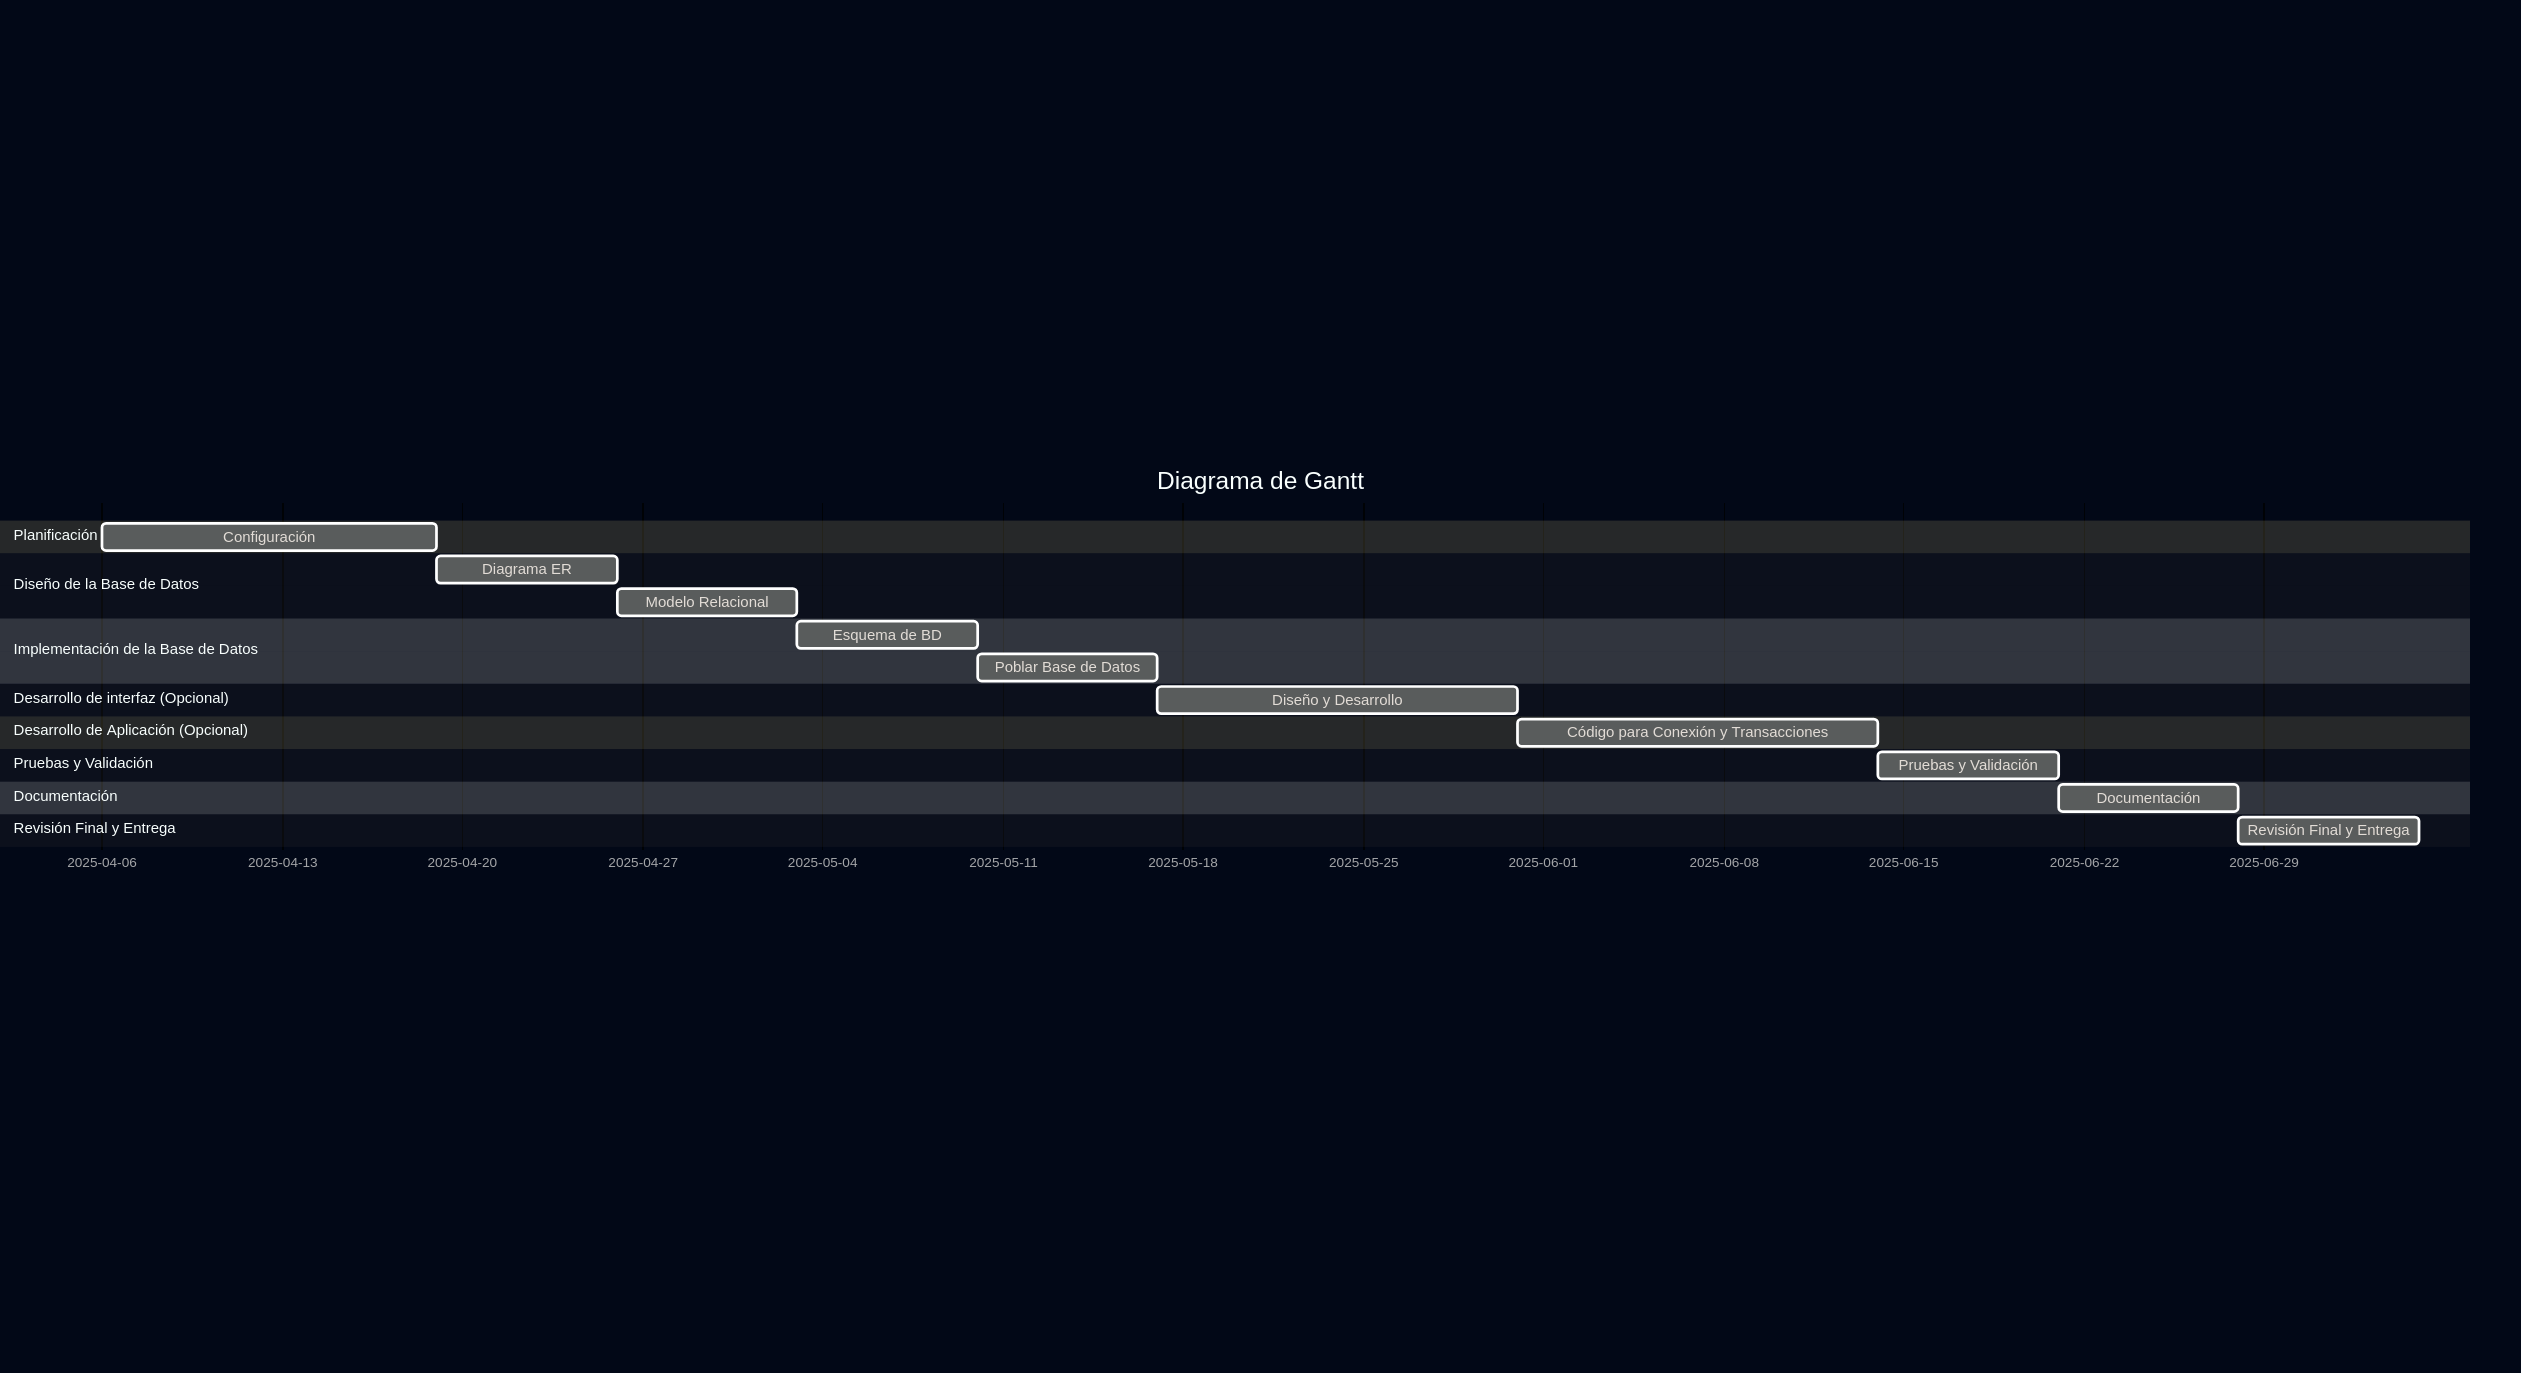
\includegraphics[width=\textwidth]{gantt.png}
    \caption{Diagrama de actividades}
\end{figure}

\newpage

\subsection{Diseño de la base de datos}
En el diseño se establece cómo se organizan, almacenan y relacionan los datos necesarios para las operaciones de la biblioteca. este diseño se desarrolló utilizando un enfque estructurado que comenzó con modelo entidad relación y se transformó en esquema relacional, implementado en PostgreSQL.

\subsubsection{Modelo entidad relación}
Es la representación más visula para las principales entidades del sistema y sus interrelaciones, con las entidades siendo:
\begin{itemize}
 \item Libros
 \item Autores
 \item Préstamos
 \item Reservas
 \item Editoriales y categorías
\end{itemize}

\subsubsection{Esquema relacional}
El ERD se convirtió en esquema relacional con tablas como:

\begin{description}
 \item [BOOKS] Almacena datos de los libros, con \textit{book id} como clave primaria
 \item [AUTHORS] Contiene información de los autores, con \textit{author id}
 \item [MEMBERS] Registra a los usuarios, con \textit{member id}
 \item [LOANS] Gestiona los préstamos, vinculando \textit{book id} y \textit{member id} mediante claves foráneas.
\end{description}

\begin{figure}[htbp]
    \centering
    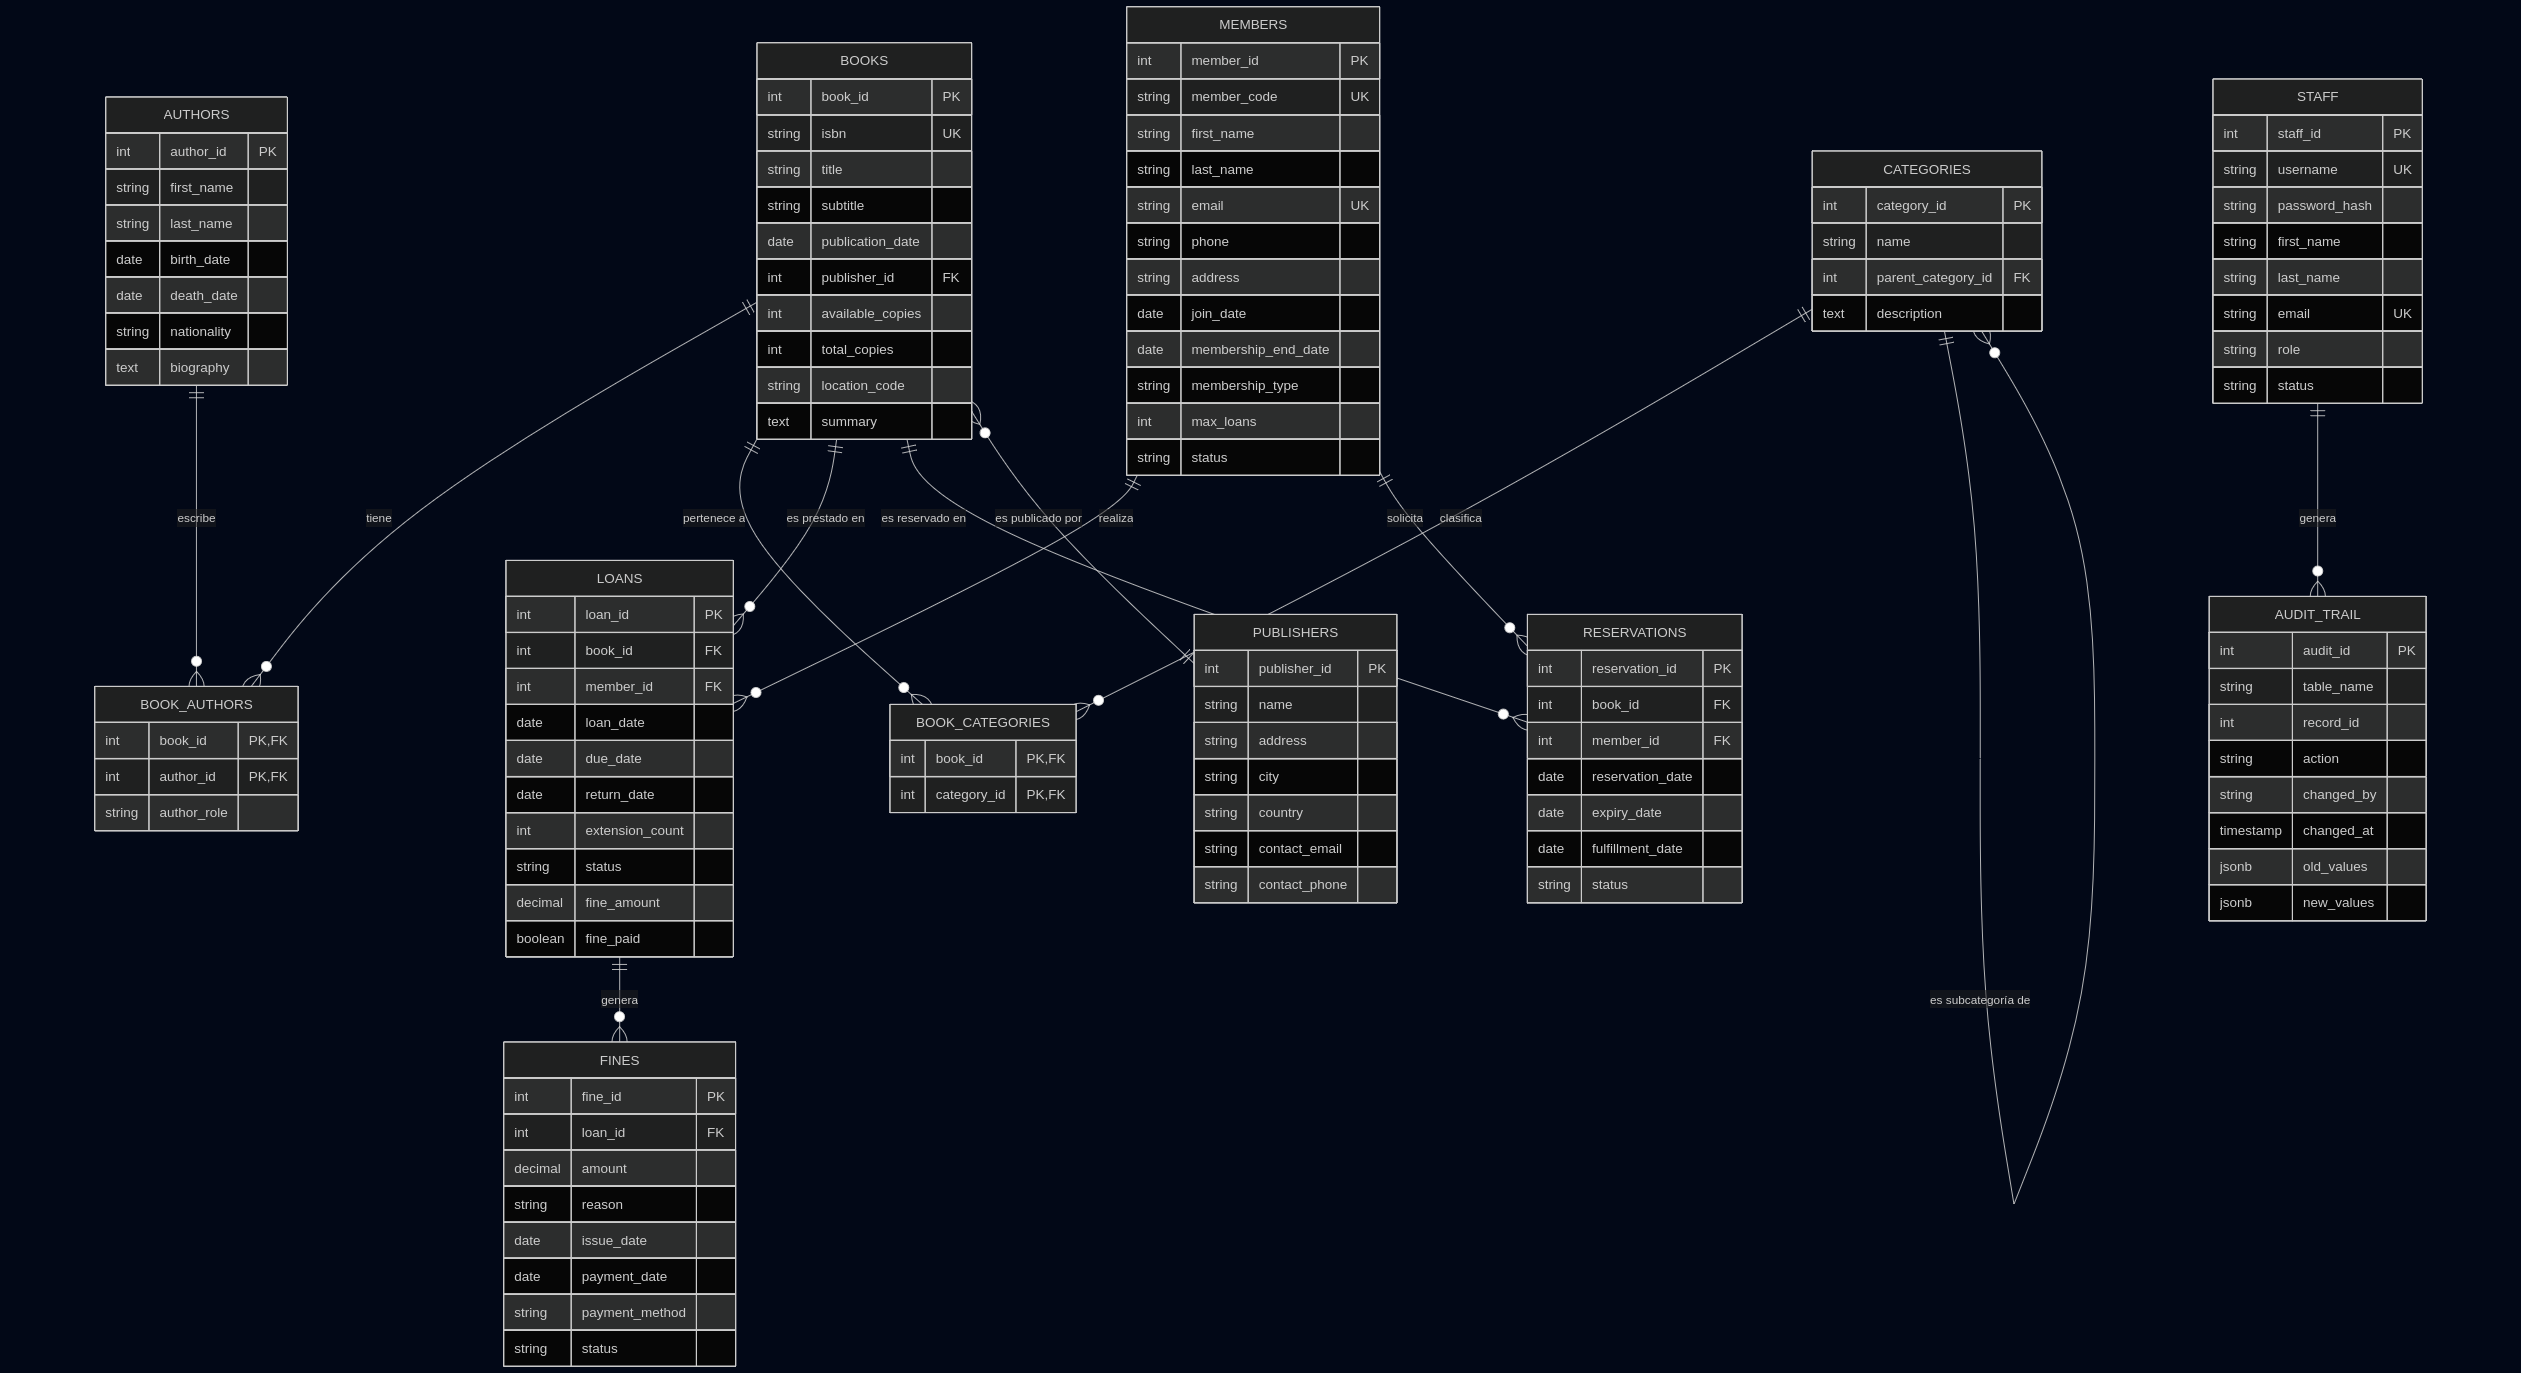
\includegraphics[width=\textwidth]{diagrama.png}
    \caption{Esquema relacional}
\end{figure}

\subsection{Implementación}
Se centró en la construcción de una base de datos relacional utilizando PostgreSQL, elegido por su robustez, capacidad de escalabilidad y soporte para operaciones complejas.

\subsubsection{Creación de la base de datos}
El proceso comenzó con la ejecución de scripts SQL para definir la estructura de la base de datos. Los scripts abarcaron:

\begin{description}
 \item [Tablas] Se crearon tablas para las entidades principales, tales como BOOKS, AUTHORS, MEMBERS, LOANS y RESERVATIONS.
 \item [Claves primarias] Se asignaron identificadores únicos a cada tabla para garantizar la unicidad de los registros.
 \item [Claves foráneas] Se establecieron relaciones entre tablas (por ejemplo, vinculando LOANS con BOOKS y MEMBERS) para mantener la integridad referencial.
 \item [Restricciones] Se aplicaron reglas como NOT NULL y CHECK para asegurar la consistencia de los datos, por ejemplo, evitando fechas de devolución inválidas.
\end{description}

PostgreSQL fue seleccionado como el sistema de gestión de bases de datos por su capacidad de manejar grandes volúmenes de datosy su compatibildad con consultas avanzadas lo que lo hace ideal para el sistema.

\subsubsection{Configuración del entorno de desarrollo}
\begin{itemize}
 \item Se utilizaron contenedores podman para aislar los entornos de desarrollo, facilitando la portabilidad y la reaplicación del sistema en diferentes máquinas.
 \item Se instaló postgreSQL en el sistem a local, utilizando la versión más reciente para aprovechar sus mejoras de rendimiento y seguridad.
\end{itemize}

A continuación, se mostrará el schema utilizado para la creación de la base de datos.

\begin{lstlisting}
-- Crear la tabla PUBLISHERS primero, ya que es referenciada por BOOKS
CREATE TABLE PUBLISHERS (
    publisher_id SERIAL PRIMARY KEY,
    name VARCHAR(100),
    address TEXT,
    city VARCHAR(50),
    country VARCHAR(50),
    contact_email VARCHAR(100),
    contact_phone VARCHAR(20)
);

-- Crear la tabla AUTHORS
CREATE TABLE AUTHORS (
    author_id SERIAL PRIMARY KEY,
    first_name VARCHAR(50),
    last_name VARCHAR(50),
    birth_date DATE,
    death_date DATE,
    nationality VARCHAR(50),
    biography TEXT
);

-- Crear la tabla CATEGORIES (auto-referenciada para categorias jerarquicas)
CREATE TABLE CATEGORIES (
    category_id SERIAL PRIMARY KEY,
    name VARCHAR(50),
    parent_category_id INTEGER,
    description TEXT,
    FOREIGN KEY (parent_category_id) REFERENCES CATEGORIES(category_id)
);

-- Crear la tabla BOOKS
CREATE TABLE BOOKS (
    book_id SERIAL PRIMARY KEY,
    title VARCHAR(255),
    genre VARCHAR(50),
    publication_date DATE,
    publisher_id INTEGER,
    available_copies INTEGER,
    location_code VARCHAR(50),
    summary TEXT,
    FOREIGN KEY (publisher_id) REFERENCES PUBLISHERS(publisher_id)
);

-- Crear la tabla BOOK_AUTHORS para la relacion muchos-a-muchos entre BOOKS y AUTHORS
CREATE TABLE BOOK_AUTHORS (
    book_id INTEGER,
    author_id INTEGER,
    PRIMARY KEY (book_id, author_id),
    FOREIGN KEY (book_id) REFERENCES BOOKS(book_id),
    FOREIGN KEY (author_id) REFERENCES AUTHORS(author_id)
);

-- Crear la tabla BOOK_CATEGORIES para la relacion muchos-a-muchos entre BOOKS y CATEGORIES
CREATE TABLE BOOK_CATEGORIES (
    book_id INTEGER,
    category_id INTEGER,
    extension_count INTEGER,
    PRIMARY KEY (book_id, category_id),
    FOREIGN KEY (book_id) REFERENCES BOOKS(book_id),
    FOREIGN KEY (category_id) REFERENCES CATEGORIES(category_id)
);

-- Crear la tabla MEMBERS
CREATE TABLE MEMBERS (
    member_id SERIAL PRIMARY KEY,
    first_name VARCHAR(50),
    last_name VARCHAR(50),
    email VARCHAR(100),
    phone VARCHAR(20),
    address TEXT,
    join_date DATE,
    membership_end_date DATE,
    membership_type VARCHAR(20),
    max_loans INTEGER,
    status VARCHAR(20)
);

-- Crear la tabla LOANS
CREATE TABLE LOANS (
    loan_id SERIAL PRIMARY KEY,
    book_id INTEGER,
    member_id INTEGER,
    loan_date DATE,
    due_date DATE,
    return_date DATE,
    FOREIGN KEY (book_id) REFERENCES BOOKS(book_id),
    FOREIGN KEY (member_id) REFERENCES MEMBERS(member_id)
);

-- Crear la tabla FINES
CREATE TABLE FINES (
    fine_id SERIAL PRIMARY KEY,
    loan_id INTEGER,
    amount DECIMAL(10,2),
    reason VARCHAR(255),
    issue_date DATE,
    payment_date DATE,
    status VARCHAR(20),
    FOREIGN KEY (loan_id) REFERENCES LOANS(loan_id)
);

-- Crear la tabla RESERVATIONS
CREATE TABLE RESERVATIONS (
    reservation_id SERIAL PRIMARY KEY,
    book_id INTEGER,
    member_id INTEGER,
    reservation_date DATE,
    expiry_date DATE,
    status VARCHAR(20),
    FOREIGN KEY (book_id) REFERENCES BOOKS(book_id),
    FOREIGN KEY (member_id) REFERENCES MEMBERS(member_id)
);

-- Crear la tabla STAFF
CREATE TABLE STAFF (
    staff_id SERIAL PRIMARY KEY,
    username VARCHAR(50),
    password_hash VARCHAR(255),
    first_name VARCHAR(50),
    last_name VARCHAR(50),
    email VARCHAR(100),
    role VARCHAR(20),
    status VARCHAR(20)
);

-- Crear la tabla AUDIT_TRAIL
CREATE TABLE AUDIT_TRAIL (
    audit_id SERIAL PRIMARY KEY,
    table_name VARCHAR(50),
    record_id INTEGER,
    action VARCHAR(20),
    changed_by VARCHAR(50),
    changed_at TIMESTAMP,
    old_values JSONB,
    new_values JSONB
);
\end{lstlisting}

\newpage

\subsection{Diagrama de flujo del sistema}
\begin{figure}[htbp]
    \centering
    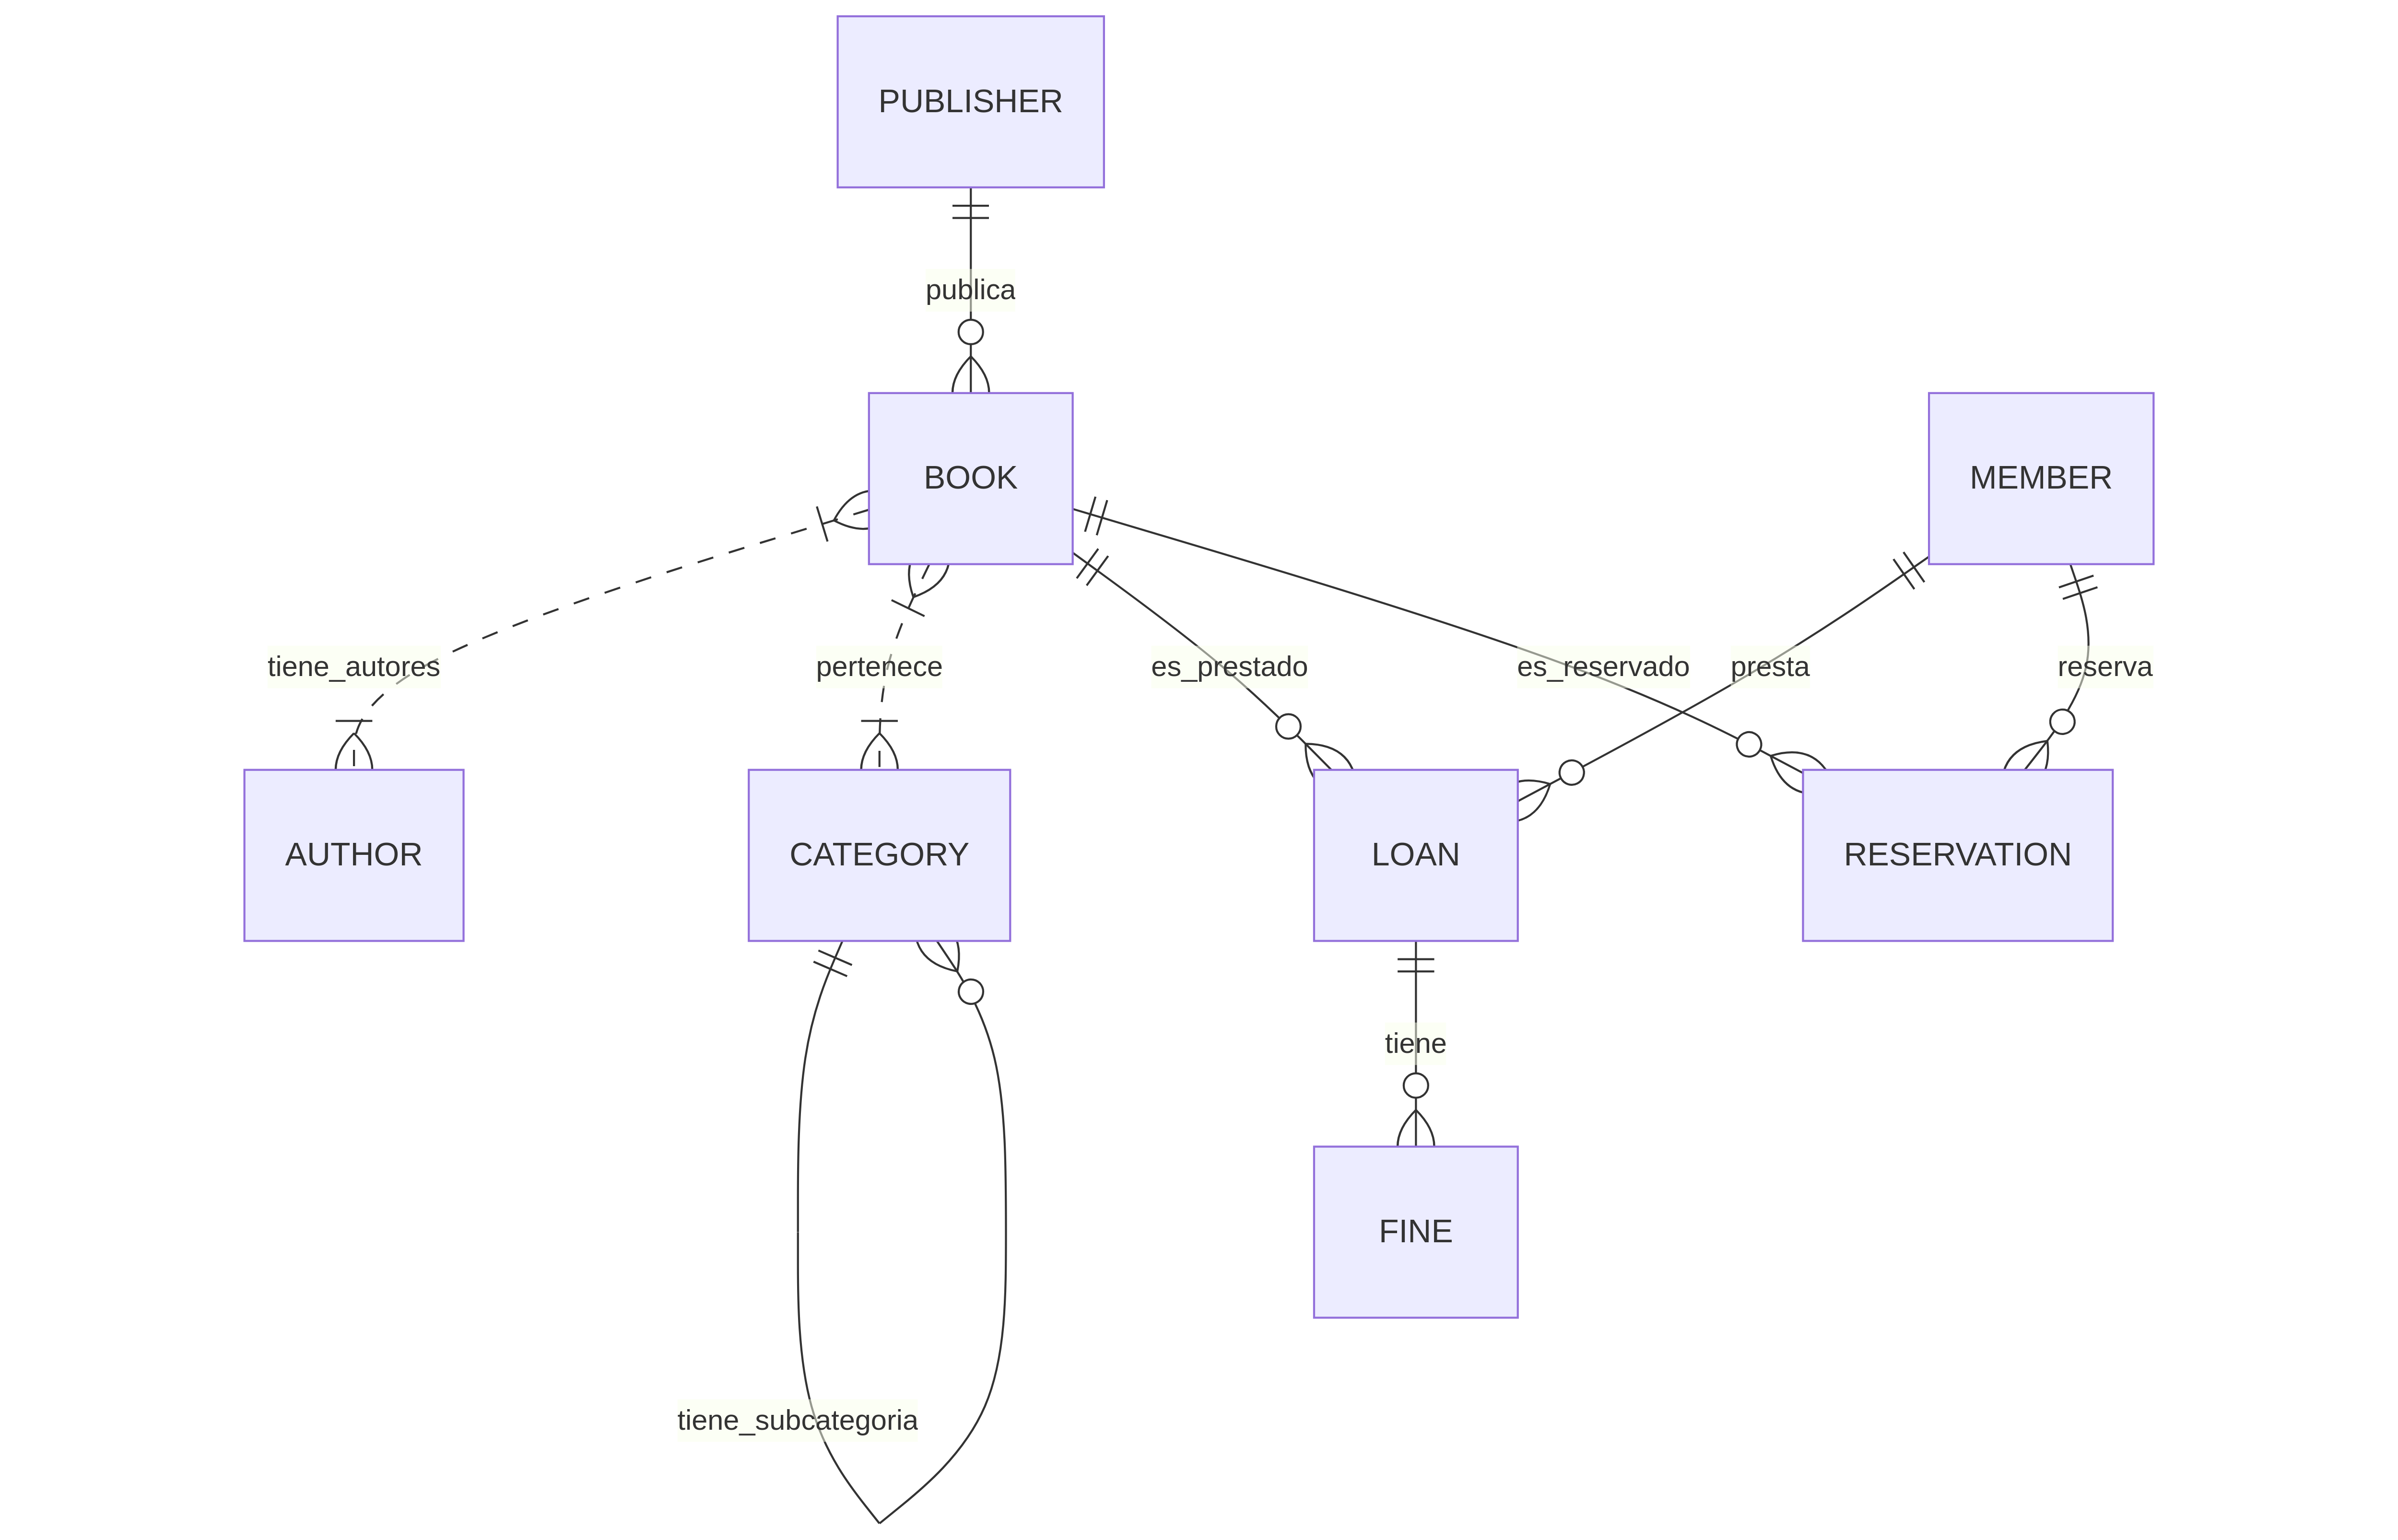
\includegraphics[width=\textwidth]{ER.png}
    \caption{Diagrama de flujo del sistema}
\end{figure}

\newpage

\subsection{Mockups}
A continuación, una demostración general de cómo podría verse una aplicación de dicho sistema de gestión de una biblioteca.
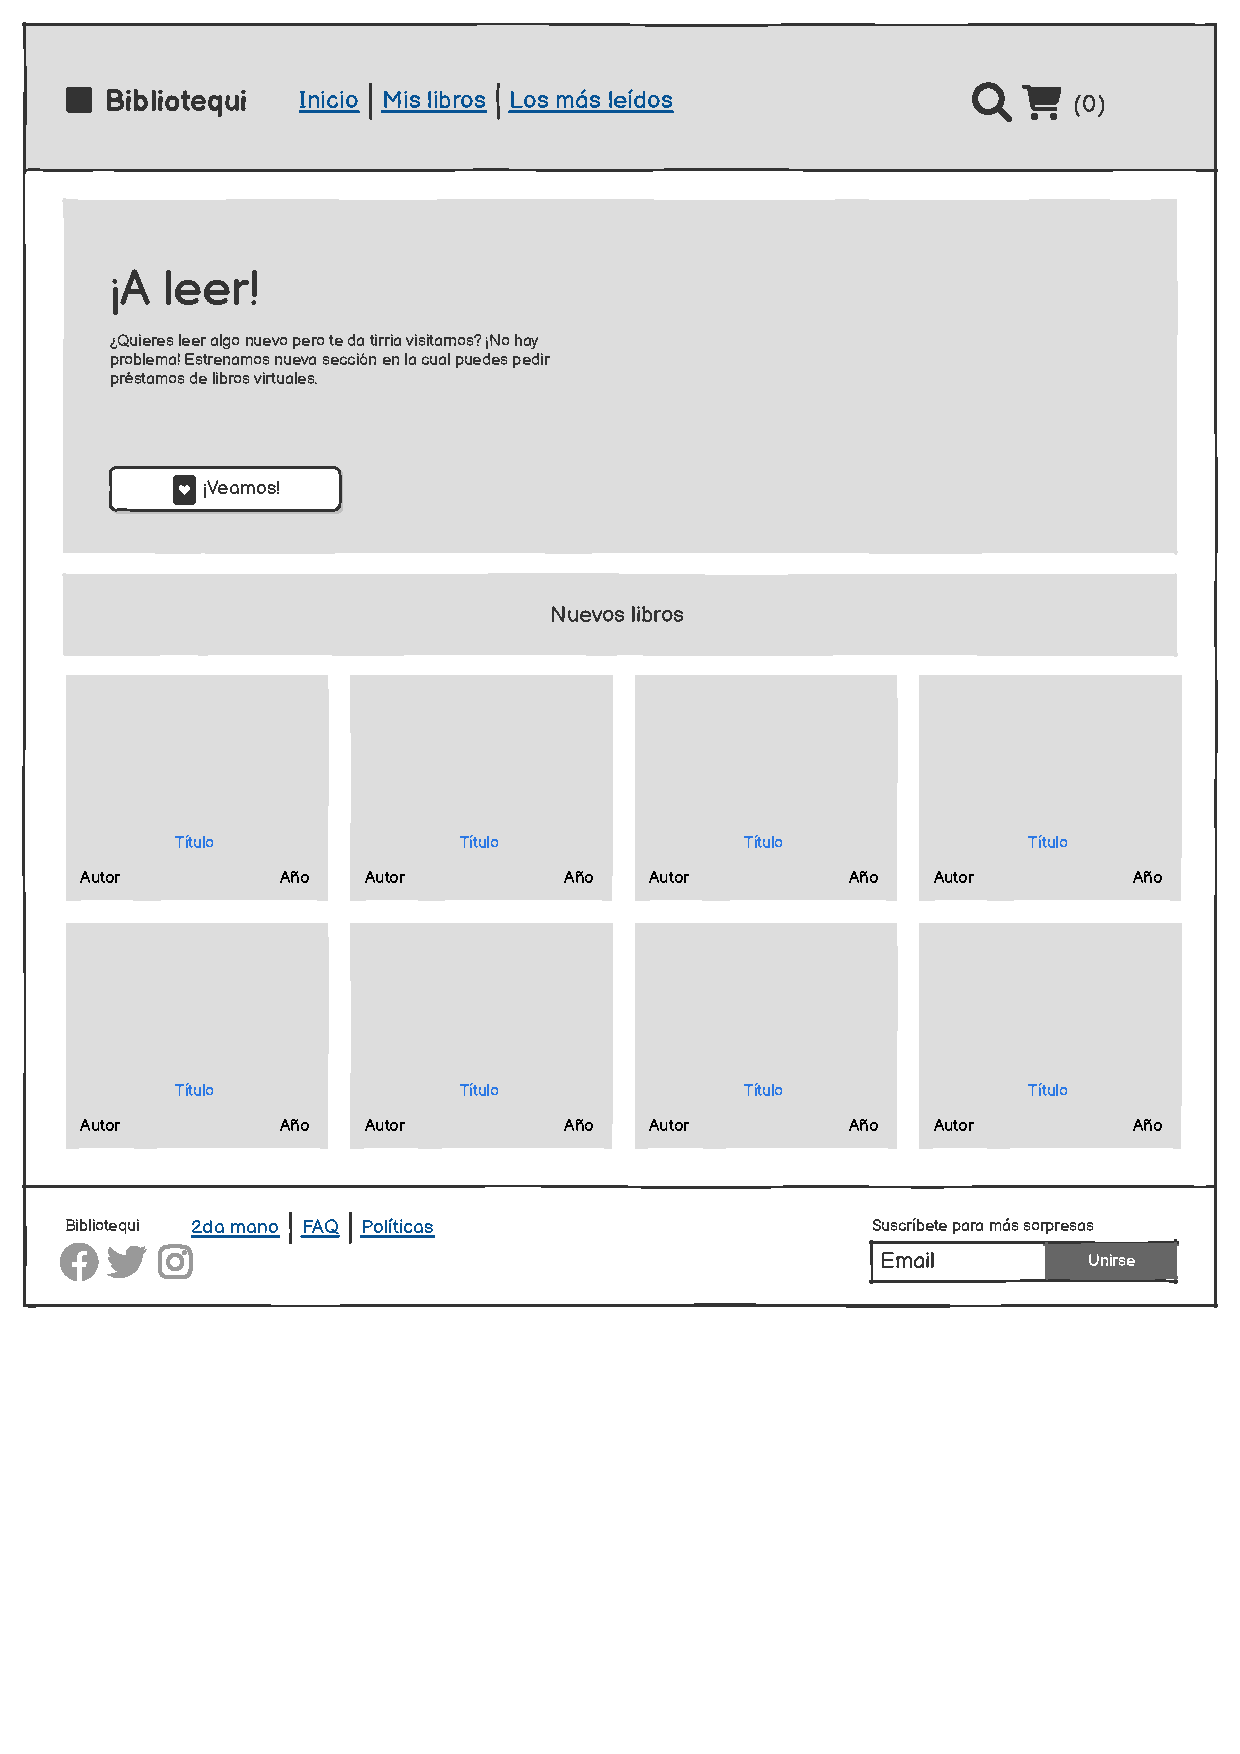
\includepdf[pages=-]{/home/ddominguez/Documents/School/7/Sem_BD/Proyecto_Final/mockup.pdf}


\section{Conclusión}
El desarrollo del sistema ha culminado en una solución integral y funcional que aborda de manera eficiente los retos de gestión de biblioteca moderna. A través de un enfoque estructurado, se logró construir un sistema capaz de adminitrar libros, miembros, préstamos y reservas.

\section{Referencias}
\begin{itemize}
\item Elmasri, R., Navathe, S. B. (2015). \textit{Fundamentals of database systems} (7th ed.). Pearson.
\item Connolly, T., Begg, C. (2014). \textit{Database systems: A practical approach to design, implementation, and management}. Pearson Education.
\end{itemize}
\end{document}
